
\section{Performance Evaluation}
\label{sec-perf}

We evaluate \app's two major components:
\sia and \pia.
%Afterwards, we compare \sia and \pia in
%a trusted auditor scenario ($\S$\ref{subsubsec-compare}).
%and the four analysis algorithms ($\S$\ref{subsubsec-compare}).
The performance evaluation was conducted on a research
cluster of $40$ workstations
equipped with Intel Xeon Quad Core HT 3.7 GHz CPU
and 16 GB RAM~\cite{zoo}.

\subsection{\sia: Efficiency v.s. Accuracy}
\label{subsec-performance}

\begin{figure*}[tbp]
\centering
\subfloat[Topology A: $1,344$ devices.]{
    \label{subfig-configA}
    \begin{minipage}[t]{0.74\textwidth}
    \centering
        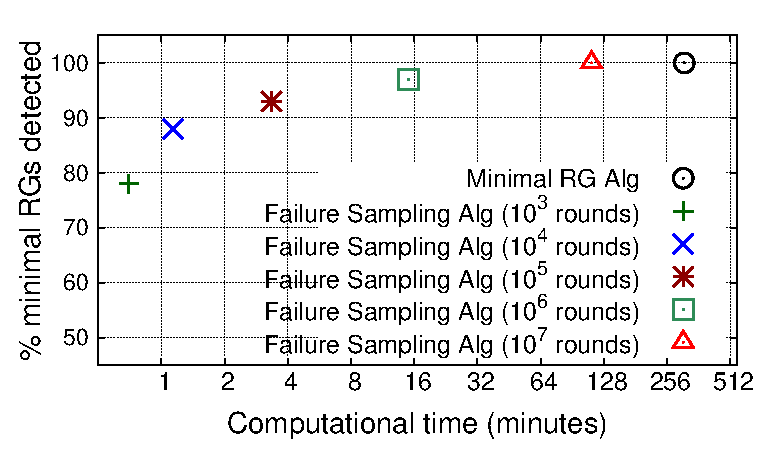
\includegraphics[width=1\textwidth]{figs/case1.eps}
    \end{minipage}
}\\\subfloat[Topology B: $4,176$ devices.]{
    \label{subfig-configB}
    \begin{minipage}[t]{0.74\textwidth}
    \centering
        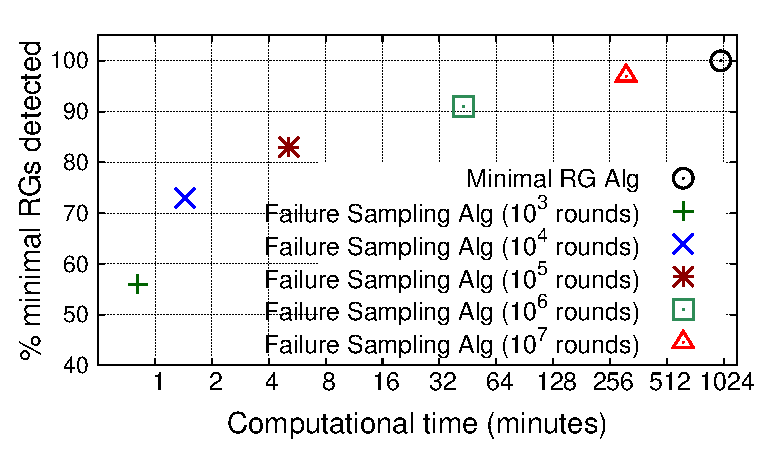
\includegraphics[width=1\textwidth]{figs/case2.eps}
    \end{minipage}
}\\\subfloat[Topology C: $30,528$ devices.]{
    \label{subfig-configC}
    \begin{minipage}[t]{0.74\textwidth}
    \centering
        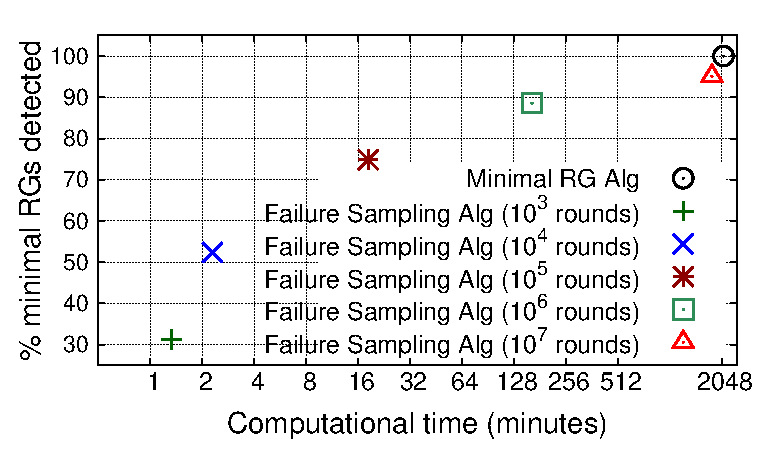
\includegraphics[width=1\textwidth]{figs/case3.eps}
    \end{minipage}
}\caption[Comparison between two algorithms of \sia.]{Performance 
  evaluation of the minimal \rg algorithm
  and the failure sampling algorithm in \sia.}
\label{fig-simulation}
\end{figure*}

We first explore the efficiency/accuracy
trade-off between \sia's
two algorithms for analyzing a dependency graph:
the minimal \rg algorithm and
the failure sampling algorithm (see $\S$\ref{sec-determine}).
The former is able to produce a complete
set of all minimal \rgs but does so within NP-hard complexity.
The failure sampling algorithm, on the other hand,
cannot guarantee completeness
but runs in linear time.
We generate three topologies
from a small-scale cloud deployment
to a large-scale deployment,
based on the three-stage
fat tree model~\cite{mysore09portland}.
These topologies include the typical components within
a commercial data center: servers, Top-of-Rack (ToR) switches,
aggregation switches, and core routers.
Table~\ref{tab-conf} gives the detail of these generated topologies.
%We run the experiments on a
%Dell Precision T3600 workstation
%equipped with Intel Xeon E5-1620 v2 Quad Core HT 3.7 GHz CPU
%and 16 GB memory.


\begin{table}[tbp]
	\centering
	\caption{Configurations of the generated topologies.}
%	\vspace{-0.15cm}		
	\begin{tabular}{l|r|r|r}
    \hline
    ~ &
    Topology A &
    Topology B &
    Topology C \\
    \hline
    \# switch ports & 16 & 24 & 48 \\
    \# core routers & 64 & 144 & 576 \\
    \# agg switches & 128 & 288 & 1,152 \\
    \# ToR switches & 128 & 288 & 1,152 \\
    \# servers & 1,024 & 3,456 & 27,648 \\
    \hline
    {Total \# devices} & 1,344 & 4,176 & 30,528 \\
    \hline
  \end{tabular}
  \label{tab-conf}
\end{table}


We compare the computational overhead
of the accurate but NP-hard minimal \rg algorithm
to that of the failure sampling algorithm with various sampling rounds ($10^3$ to $10^7$).
Figure~\ref{fig-simulation} shows the result that
%With the minimal \rg algorithm as a baseline,
%we evaluated accuracy versus run-times
%for the failure sampling algorithm.
the failure sampling algorithm
runs much more efficiently than the minimal \rg algorithm while achieving a reasonably high accuracy.
For example, in topology B, the failure sampling algorithm
uses 90 minutes to detect 92\% of all the minimal \rgs
with $10^6$ sampling rounds,
in comparison to 1046 minutes for the minimal \rg algorithm.
%In the last two configurations,
%the failure sampling algorithm (with $10^6$ rounds)
%balances performance and accuracy better than the ones (with $10^5$
%and $10^7$ rounds) and minimal cut set algorithm.
%; thus, we suggest that
%the failure sampling algorithm with $10^6$ rounds is the most
%suitable to auditing large scale clouds.


\subsection{\pia: System Overheads}
\label{subsec-micro}

\begin{figure}[tb] \centering
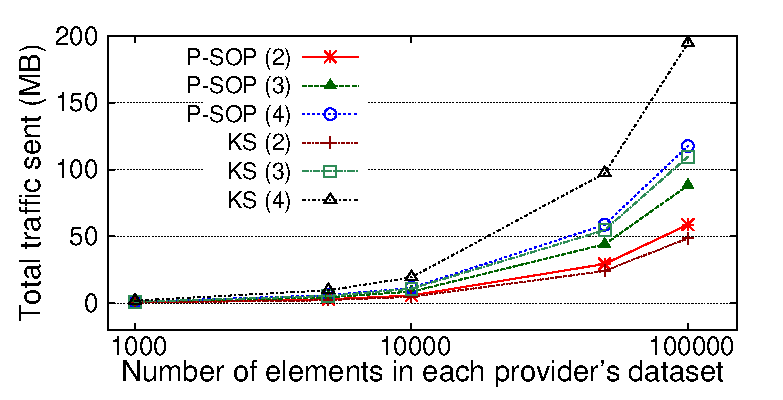
\includegraphics[width=0.96\textwidth]{figs/net.eps}
\caption[Bandwidth overhead evaluation of \pia]{Bandwidth
  overhead evaluation of \pia.  \pso($k$) and KS($k$) mean
  that there are $k$ cloud providers participating in the \pso and KS
  protocols, respectively. The commutative encryption in \pso 
  uses a 1024-bit key, and the homomorphic encryption in KS also 
  uses a 1024-bit key.}
\label{fig-net}
\end{figure}

To better understand the performance of \pia, 
we compare \pso with KS from both aspects of bandwidth and computation.

For a private independence auditing system,
the cryptographic operations tend to be
the major bandwidth and computational bottleneck.
Thus, we evaluate the performance of \pia
by comparing the bandwidth and computational overheads of 
\pso protocol with KS protocol.
Specifically, the cryptographic primitives of \pso
are hashing, commutative encryption, and permutation.
The KS protocol is mainly built on hashing, homomorphic crypto operations,
and permutation.

In the evaluation, there are $k$ cloud providers
with $n$ elements in each provider's local dataset.
We set $k$ to $2$, $3$ and $4$,
and vary $n$ between $1,000$ and $100,000$ to 
cover a wide range of real-world settings.
We measure and compare \pso with KS in terms of their
bandwidth and computational overheads at each such cloud provider.
Figure~\ref{fig-net} and \ref{fig-com}
show the bandwidth overhead and computational overhead, respectively.
%\pso (i) and KS (i) in both figures mean
%$i$ providers who coordinately perform the protocols.

With a small number of cloud providers (\eg, $k=2$),
the bandwidth overhead of KS is comparable to that of \pso.
However, with an increasing number of cloud providers,
KS's bandwidth overhead increases much faster than \pso's.
With respect to the computational overhead,
\pso outperforms KS by a few orders of magnitude although both protocols' computational overheads increase almost linearly with the number of elements in each cloud provider's dataset.
Altogether, the evaluation shows that our PIA system
can efficiently handle large
cloud providers each with even hundreds of thousands of system components.

\begin{figure}[tb] \centering
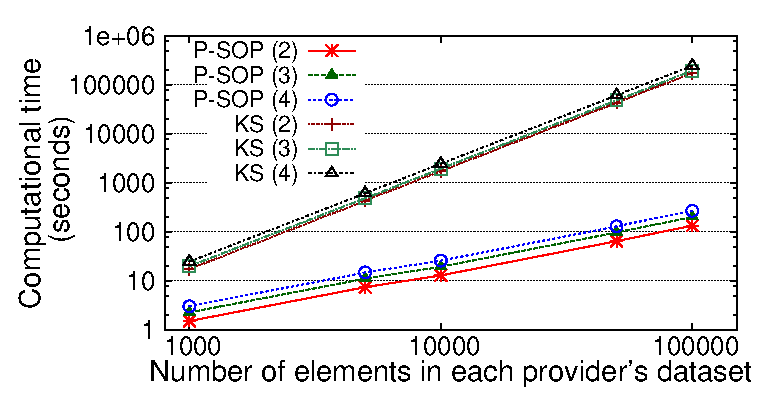
\includegraphics[width=0.96\textwidth]{figs/com.eps}
\caption[Computational overhead evaluation of \pia]{Computational
  overhead evaluation of \pia.  \pso($k$) and KS($k$) mean
  that there are $k$ cloud providers participating in the \pso and KS
  protocols, respectively. The commutative encryption in \pso 
  uses a 1024-bit key, and the homomorphic encryption in KS also 
  uses a 1024-bit key.}
\label{fig-com}
\end{figure}



%We now compare \pso with KS in terms of
%their computational and bandwidth overheads
%at each cloud provider,
%which is the bottleneck of the whole system.
%In this evaluation, there are $k$ providers (replicas) ran
%both \pso and KS protocols
%with $n$ elements in each of their data sets.
%We vary $n$ between $1,000$ and $100,000$,
%and set $k$ to $2$, $3$ and $4$ respectively.
%The computational and bandwidth overhead
%are the same as the definitions
%of measuring microbenchmarks.\abbr{}{, \ie,
%all the time required by cryptographic operations
%and the size of encrypted messages sent.}
%Figure~\ref{subfig-net} and Figure~\ref{subfig-com}
%show each provider's bandwidth and
%computational overhead, respectively.
%For computational overhead, \pso is much efficient than KS.
In particular, in a three redundancy deployment,
an alternative service provider owning
a local data set with $100,000$ elements can finish all
the computation operations with about $200$ seconds,
if the provider is using \pso.
Regarding bandwidth, we concede KS protocol
is less than \pso in the two redundancy deployment case.
However, \pso is more efficient than KS
in other two cases.
%To illustrate \pia's performance gains and scalability,

\begin{figure*}[tbp] \centering
\subfloat[Two-way redundancy.]{
    \label{subfig-2rep}
    \begin{minipage}[t]{0.84\textwidth}
    \centering
        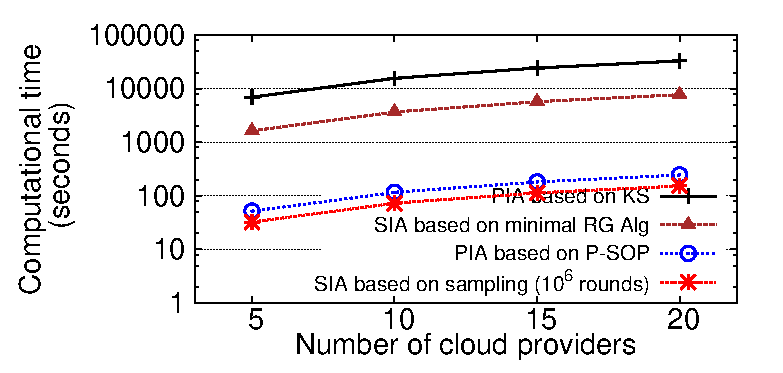
\includegraphics[width=1\textwidth]{figs/2-10000-way.eps}
    \end{minipage}
}\\ \subfloat[Three-way redundancy.]{
    \label{subfig-3rep}
    \begin{minipage}[t]{0.84\textwidth}
    \centering
        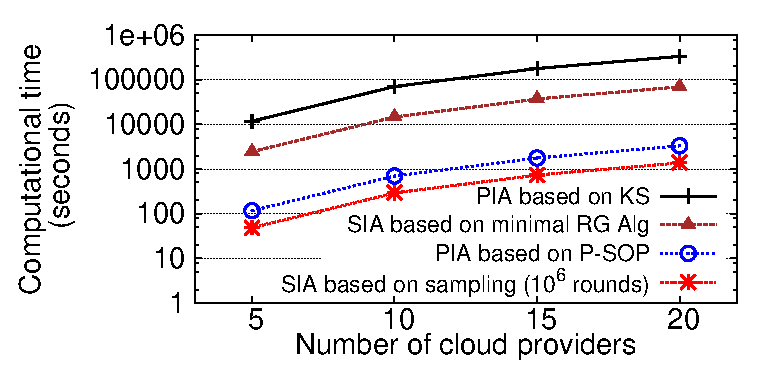
\includegraphics[width=1\textwidth]{figs/3-10000-way.eps}
    \end{minipage}
}
\caption[Comparison between \sia and \pia.]{Performance 
  comparison between \sia and \pia.
  Each cloud provider maintains a 10,000-element dataset.}
\label{fig-compare}
\end{figure*}


\subsection{Comparison: \sia Versus \pia}
\label{subsec-compare}

Compared with the \sia where there is a trusted auditor, 
we would also like to understand
how much extra overhead the \pia approach incurs
to preserve the secrecy of each participating cloud provider's data.
%construct two scenario
%where there are $n$ individual cloud providers
%and a trusted auditor (\eg, a cloud consulting company).
Assume each cloud provider maintains a local dataset
containing $10,000$ elements.
To preserve secrecy for each cloud provider, an auditing client
%an application-level service provider (\ie, client)
relies on either the \pia system or the comparable KS-based system
to determine the most independent redundancy deployment.
For a comparison, we also assume another setting where
there exists a trusted auditor who knows all cloud providers' datasets.  
This trusted auditor runs
\sia at the component-set level of detail based on
the minimal \rg algorithm or the failure sampling algorithm
with $10^6$ rounds.
%in order to produce auditing reports.

The motivation we construct the above scenario is to compare our
auditing algorithms in a ``hybrid'' auditing task case.
Our experiments measure computational
by changing $n=5, 10, 15$ and $20$~($n$ is the number of
alternative cloud providers).
We assume that the trusted auditor,
can get all cloud providers' datasets,
then generates a dependency graph at component-set
level of detail with the collected data,
and finally performs the auditing algorithms on the graph.

Figure~\ref{subfig-2rep} and \ref{subfig-3rep}
show the computational overheads of these independence calculations
for all potential two- and three-way redundancies, respectively.
As shown in Figure~\ref{subfig-2rep} and Figure~\ref{subfig-3rep}, 
preserving the secrecy of cloud providers' data does incur extra overhead.
Surprisingly, this cost is not as high as might be expected:
we see that the computational
overhead of ``\pia based on \pso'' is less than
twice that of ``\sia based on sampling ($10^6$ rounds)''.
The \sia sampling scheme does implement a more general analysis than \pia,
supporting fault graphs rather than just component sets.
Unsurprisingly, both ``\pia based on KS''
and ``\sia based on minimal \rg Alg'' do not scale well.
%We observe that the failure sampling algorithm with $10^6$ rounds
%has the best performance and KS needs the longest running time.
%We also did similar evaluations on data sets with $1,000$
%and $5,000$ items respectively.


